\documentclass[a4paper,norsk,12pt]{article}
\usepackage[utf8]{inputenc}

% Oppsett for norsk
\usepackage[norsk]{babel}
\usepackage{times}
\usepackage[T1]{fontenc}
\usepackage{parskip}
\DeclareUnicodeCharacter{00A0}{ }
\newcommand{\strek}{\textthreequartersemdash}

% Andre pakker
\usepackage{oving}
\usepackage{amsmath}
\usepackage{amssymb}
\usepackage{varioref}
\usepackage{subcaption}
\usepackage{units}
\usepackage{todo}

\def \oppgavename {Problem}

% Roman numerals
\makeatletter
\newcommand*{\rom}[1]{\expandafter\@slowromancap\romannumeral #1@}
\makeatother


\title{MAT200 --- Mathematical Methods 2}
\subtitle{Compulsory Assignment 1}
\author{Christian Stigen}
\date{UiS, 19.~februar, 2016}

\begin{document}
\maketitle

\oppgave{1 (i)}
\label{problem.1}

The radicand must be zero or greater, or
\begin{align*}
  0 & \leqslant x^2-6x+\frac{1}{4}y^2 \> \Big{|} \cdot-4 \\
  0 & \geqslant 4x(6-x)-y^2 \\
  y^2 & \geqslant 4x(6-x)
\end{align*}
The right-hand side is zero for $x=0$ and $x=6$, and negative for $x<0$
and $x>6$. Thus, the inequality is true for $0 < x < 6$.

For plotting $\mathcal{D}(f)$, we note that
\begin{align*}
  y_{-} \leqslant -2\sqrt{x(6-x)} & \wedge y_{+} \geqslant 2\sqrt{x(6-x)}
  \,\text{for}\, 0<x<6
\end{align*}
In fact, taken together, they form an ellipse (see figure \vref{plot.p1}).

\begin{figure}[htp]
  \centering
  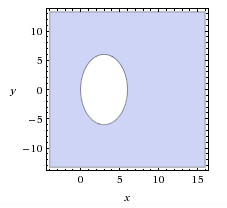
\includegraphics{ob1plot.png}
  \caption{Plot of $\mathcal{D}(f)$ in problem 1 (i).}
  \label{plot.p1}
\end{figure}

\oppgave{1 (ii)}

This is the same as solving $f=0$ and $f=4$, or

\begin{align*}
  f(x,y) &= 0 \\
  \sqrt{x^2 - 6x + \frac{1}{4}y^2} &= 0\\
  x^2 - 6x + \frac{1}{4}y^2 &= 0\\
  y^2 = -4(x^2 - 6x) &= 4x(6-x) \\
  \\
  f(x,y) &= 4 \\
  \sqrt{x^2 - 6x + \frac{1}{4}y^2} &= 4\\
  x^2 - 6x + \frac{1}{4}y^2 &= 16 \\
  y^2 = -4\left(x^2 - 6x - 16\right) &= -4(x-8)(x+2) \\
\end{align*}

By the previous results, for $f=0$ we get $y = \pm 2\sqrt{4x(6-x)}$, which is
the same ellipse as we got in (ii). See \vref{plot.p2}.

\begin{figure}[htp]
  \centering
  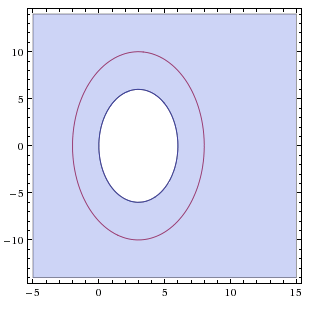
\includegraphics{ob1plot2.png}
  \caption{Plot of $f=0$ and $f=4$ in problem 1 (ii).}
  \label{plot.p2}
\end{figure}


\oppgave{1 (iii)}

\oppgave{2 (i)}

\oppgave{2 (ii)}

\oppgave{2 (iii)}

\oppgave{3 (i)}

\oppgave{3 (ii)}

\oppgave{3 (iii)}

\oppgave{3 (iv)}

\begin{align*}
  F(0,y) &= 1 \\
  2y \sin^2(-\frac{\pi}{4}) &= 1 \\
  2y\frac{1}{2} &= 1 \\
  y &= 1 \\
  F(0,1) &= 1
\end{align*}

\end{document}
